\documentclass{beamer}
\usepackage{float}
% Define the theme and color scheme
\usetheme{Goettingen}
\usecolortheme{seahorse}

% Define the title, author, and date
\title{Group 5: Euler's Method}

\begin{document}

% Create the title slide
\begin{frame}
  \titlepage
  \begin{center}
  \textbf{Ashraf Mohammed Hassan Anil}: \textit{SCT211-0255/2021}
  
  \textbf{Yunus Mohamed Abdi}: \textit{SCT211-0720/2021}
  
  \textbf{Yusin Ali Adan}: \textit{SCT211-0655/2021}
  \end{center}
\end{frame}

% Create the slide with Euler's Method description
\begin{frame}
  \frametitle{Description of Euler's Method}
Euler's Method is a numerical method used in numerical analysis for solving ordinary differential equations (ODEs) with a given initial value. It is named after the mathematician Leonhard Euler who developed the method in the 18th century.

The basic idea of Euler's method is to approximate the solution to the ODE by using the tangent line at the initial point to make a local linear approximation of the solution. Then, the solution at a small time increment from the initial point is estimated by following the tangent line for that increment.

The points are computed iteratively as follows:

$$y_{n+1} = y_n + h * f(x_n, y_n)$$

where $h$ is the time step size and $x_{n+1} = x_n + h.$
\end{frame}

% Create the slide with the step-by-step procedure
\begin{frame}
  \frametitle{Step by Step procedure}
  \begin{enumerate}
    \item Given an initial value problem of the form $y' = f(x, y), y(x_0) = y_0, \text{choose a time step size }h.$

    \item Set $x = x_0$ and $y = y_0 as$ the initial values.

    \item Use Euler's method to compute the values $y_{n+1}$ for $n = 0, 1, \ldots, n-1$:
          \begin{align*}
            x_{n+1} &= x_n + h \\
            y_{n+1} &= y_n+ h*f'(x_n, y_n)
          \end{align*}
    \item Repeat step 3 until you reach the desired endpoint or number of time steps.
    \item Plot the graph to visualize the solution
  \end{enumerate}
\end{frame}

% Create the slide with solved example of Euler's Method
\begin{frame}
  \frametitle{Solved example}
Question: Given that $y = x^2$ and the initial points are p(1, 1) with step-size $h = 0.2$. Obtain $y(2.0)$\\[11pt]
\textbf{Solution:}

$n = (y_n - y_0) \text{divide by} h$

$n = (2.0-1)/5$
$\text{therefore: } n = 5$.The values of $x_n$ and $y_n$ will be:

\begin{table}[H]
    \centering
    \begin{tabular}{|c|c|c|c|}
        \hline
         n&$x_n$&$y_n$&Accurate  \\ \hline
         0&1&1&1  \\ \hline 
         1&1.2&1.48&1.44  \\ \hline 
         2&1.4&2.04&1.96  \\ \hline 
         3&1.6&2.68&2.56  \\ \hline 
         4&1.8&3.40&3.24  \\ \hline 
         5&2.0&4.16&4.00  \\ \hline 
    \end{tabular}
    \caption{Values of $x_n$ and $y_n$ }
    \label{tab:my_label}
\end{table}

\end{frame}

% Create the slide with the Python code
\begin{frame}[fragile]
  \frametitle{Python Code I}

  Here's an example implementation of Euler's method in Python:

  \begin{verbatim}
import matplotlib.pyplot as plt


def f(x):
    return x ** 2


def df(x):
    return 2 * x


def euler_method(f_prime, x0, y0, h, num_steps):
    x = [x0]  
    y = [y0] 
  \end{verbatim}
\end{frame}

\begin{frame}[fragile]
  \frametitle{Continuation ...}
   \begin{verbatim}

    for i in range(num_steps):
        x_i = x[i]  # Get the current time
        y_i = y[i]  # Get the current solution value
        y_next = y_i + h * f_prime(x_i)

        x_next = x_i + h

        x.append(x_next)
        y.append(y_next)

    return x, y
    \end{verbatim}
\end{frame}

\begin{frame}[fragile]
  \frametitle{Continuation ...}
   \begin{verbatim}
x_initial = 1
y_initial = 1
size_step = 0.2
n = 5

x_values, y_values = euler_method(df, x_initial, y_initial, 
size_step, n)
y_euler = y_values[-1]
y_accurate = f(x_values[-1])

for pt in range(len(x_values)):
    print(f"Value at y({x_values[pt]}) = {y_values[pt]}")

print()
print(f"Error = {y_accurate-y_euler}")
\end{verbatim}
\end{frame}

\begin{frame}[fragile]
  \frametitle{Continuation ...}
   \begin{verbatim}
x_real = [1, 1.1, 1.3, 1.4, 1.5, 1.6, 1.7, 1.8, 1.9]
y_real = [num ** 2 for num in x_values]

plt.plot(x_values, y_values, color='red',
label="Approximation with Euler's method")

plt.plot(x_values, y_real, color='blue',
label='Accurate curve')

plt.legend()
plt.xlabel('x-axis')
plt.ylabel('y-axis')
plt.grid()
plt.show()

  \end{verbatim}
\end{frame}

\begin{frame}[fragile]
  \frametitle{Output of the code with $h = 0.2$}
Value at y(1) = 1

Value at y(1.2) = 1.4

Value at y(1.4) = 1.88

Value at y(1.5999999999999999) = 2.44

Value at y(1.7999999999999998) = 3.08

Value at y(1.9999999999999998) = 3.8\\[10pt]
Error = 0.1999999999999993

\end{frame}

\begin{frame}
  \frametitle{Euler's Plot with $h = 0.2$}
  \begin{center}
    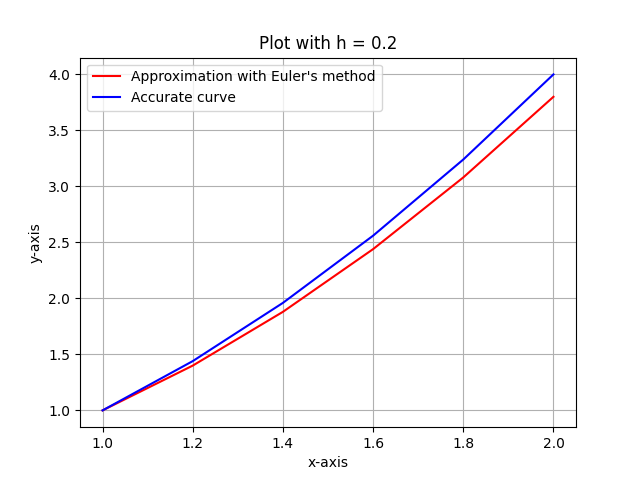
\includegraphics[width=0.8\textwidth]{Euler_02.png}
  \end{center}
\end{frame}

\begin{frame}[fragile]
  \frametitle{Output of the code when $h = 0.4$}
Value at y(1) = 1

Value at y(1.4) = 1.8

Value at y(1.7999999999999998) = 2.92

Value at y(2.1999999999999997) = 4.359999999999999

Value at y(2.5999999999999996) = 6.119999999999999

Value at y(2.9999999999999996) = 8.2\\[10pt]
Error = 0.7999999999999989

\end{frame}

\begin{frame}
  \frametitle{Euler's Plot with $h = 0.4$}
  \begin{center}
    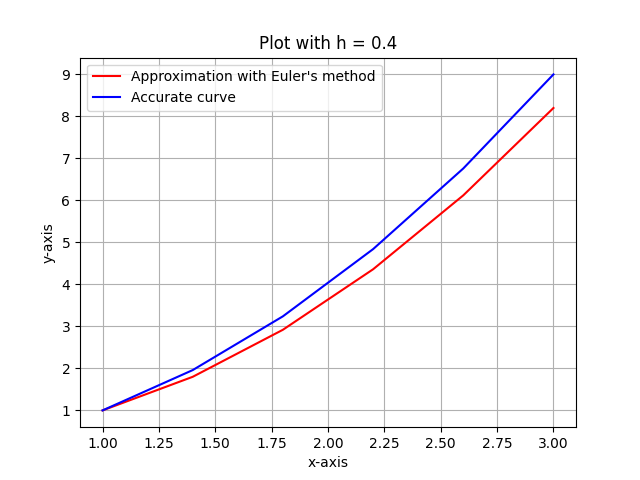
\includegraphics[width=0.8\textwidth]{Euler_04.png}
  \end{center}
\end{frame}

\begin{frame}
  \frametitle{Conclusion}
Euler's method is a \textbf{\textit{simple}} and \textbf{\textit{straightforward}} algorithm for approximating solutions to ordinary differential equations (ODEs). However:\\[11pt]
Euler's method is a \textbf{\textit{first-order method}}, meaning that the error in the approximation is \textbf{proportional to the step size h used in the algorithm.} As a result, small step sizes are required to achieve high accuracy, which can make the computation time-consuming and impractical for large-scale problems, also it can \textit{\textbf{only be applied directly to first-order ODEs.}} For higher-order ODEs, the method must be modified by transforming the higher order ODE into a system of first-order ODEs which can make the computation more complex and less efficient.Therefore, more advanced numerical methods such as the \textbf{\textit{Runge-Kutta methods}} or the \textbf{\textit{Adams-Bashforth methods}} are typically used

\end{frame}


\end{document}



